\chapter{Supporting Information: Influenza A gradual and
  epochal evolution: insights from simple models}

\author{Sébastien Ballesteros$^{1,*}$, Elisabeta Vergu$^{2}$, Bernard
  Cazelles$^{1,3}$}

%\date{}

%\renewcommand{\figurename}{Figure S}
%\renewcommand{\tablename}{Table S}

~ \\
$^1$UMR 7625  (UPMC, ENS, AgroParisTech, CNRS), Ecole Normale Supérieure, Unit of Eco-Evolutionary Mathematics,  46 rue d'Ulm, F-75230 Paris Cedex 05, France. \\
$^2$~INRA, UR341 Mathématiques et Informatique Appliquées, F-78352 Jouy en Josas, France \\
$^3$~UMMISCO UMI 209 IRD-UPMC, 93142 Bondy, France

~ \\
$^*$\textit{Corresponding author}:  \\
E-mail: sebastien.ballesteros@biologie.ens.fr

\section{Reaction scheme for the $SBRI$ model}

\begin{table}[!h]
\center
	\begin{tabular}{ll}
		reaction & rate \\
		birth\\
		$R_\varnothing \rightarrow R_\varnothing +1$ & $\mu N$ \\
		death\\
		$R_\varnothing \rightarrow R_\varnothing -1$ & $\mu R_\varnothing$ \\
		$R_1 \rightarrow R_1-1$ & $\mu R_1$ \\
		$R_1 \rightarrow R_2-1$ & $\mu R_2$ \\
		$R_{12} \rightarrow R_{12}-1$ & $\mu R_{12}$ \\
		$I^1 \rightarrow I^1-1$ & $\mu I^1$ \\
		$I^2 \rightarrow I^2-1$ & $\mu I^2$ \\
		recovery \\
		$I^1 \rightarrow I^1-1$ & $\nu I^1$ \\
		$I^2 \rightarrow I^2-1$ & $\nu I^2$ \\
		$I^1$ production and $R_1$ only immunisation from $R_\varnothing$ \\
		$R_\varnothing \rightarrow R_\varnothing-1$ ; $R_1 \rightarrow R_1+1$ ; $I^1 \rightarrow I^1+1$ & $(1-\sigma) \beta_1 R_\varnothing I^1/N$ \\
		$I^2$ production and $R_1$ only immunisation from $R_\varnothing$ \\
		$R_\varnothing \rightarrow R_\varnothing-1$ ; $R_1 \rightarrow R_1+1$ ; $I^2 \rightarrow I^2+1$ & $(1-\sigma) \beta_2 R_\varnothing I^2/N$ \\
		$I^1$ production and $R_{12}$ only immunisation from $R_\varnothing$ \\
		$R_\varnothing \rightarrow R_\varnothing-1$ ; $R_{12} \rightarrow R_{12}+1$ ; $I^1 \rightarrow I^1+1$ & $\sigma \beta_1 R_\varnothing I^1/N$ \\
		$I^2$ production and $R_{12}$ only immunisation from $R_\varnothing$ \\
		$R_\varnothing \rightarrow R_\varnothing-1$ ; $R_{12} \rightarrow R_{12}+1$ ; $I^2 \rightarrow I^2+1$ & $\sigma \beta_2 R_\varnothing I^2/N$ \\
		$I^1$ production and $R_{12}$ only immunisation from $R_1$ \\
		$R_1 \rightarrow R_1-1$ ; $R_{12} \rightarrow R_{12}+1$ ; $I^1 \rightarrow I^1+1$ &  $\beta_1 R_1 I^1/N$ \\
		$I^2$ production and $R_{12}$ only immunisation from $R_1$ \\
		$R_1 \rightarrow R_1-1$ ; $R_{12} \rightarrow R_{12}+1$ ; $I^2 \rightarrow I^2+1$ &  $\beta_2 R_1 I^2/N$ \\
		$R_{12}$ immunity acquisition from $R_1$ by $I^1$ \\
		$R_{12} \rightarrow R_{12}+1$ ; $R_1 \rightarrow R_1-1$ &  $\sigma \beta_1 R_1 I^1/N$ \\
		$R_{12}$ immunity acquisition from $R_1$ by $I^2$ \\
		$R_{12} \rightarrow R_{12}+1$ ; $R_1 \rightarrow R_1-1$ & $\sigma \beta_2 R_1 I^2/N$
	\end{tabular}
	\caption{Reaction scheme for the $SBRI$ model}
	\label{tab:reaction}
\end{table}

In the case of reduced susceptibility ($SBRS$ model), the reaction scheme of table~S\ref{tab:reaction} remains the same except that the last 2 reactions do not occur.


\clearpage

\section{Critical community size for influenza}

\begin{figure}[!h]
  \center
  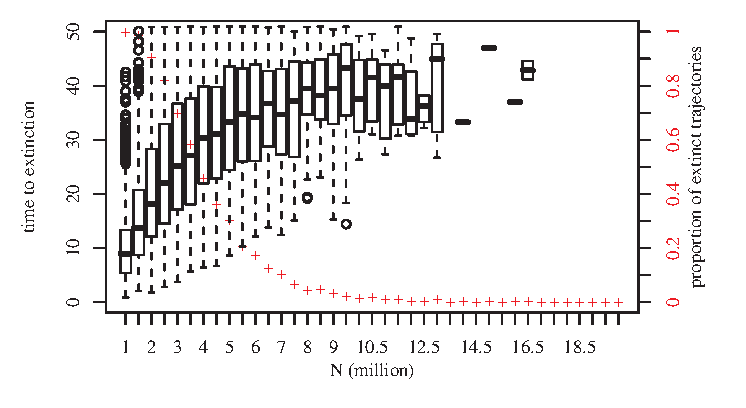
\includegraphics[]{graphs/article1/css_sir.eps}
  \caption{Endemic fadeouts obtained using the $SIR$ stochastic model
    estimated by the distribution of the time to extinction. Red
    crosses represent the proportion of extinct trajectories after
    $T_{max} = 50$ years calculated on 1000 simulations. Initial
    conditions correspond to the endemic equilibrium of the
    deterministic model: $S=200000$, $I=250$ and $R=799750$. Parameter
    values are given in Table~1 (theoretical set).}
\label{fig:ccs}
\end{figure}


\begin{figure}[!h]
  \center
  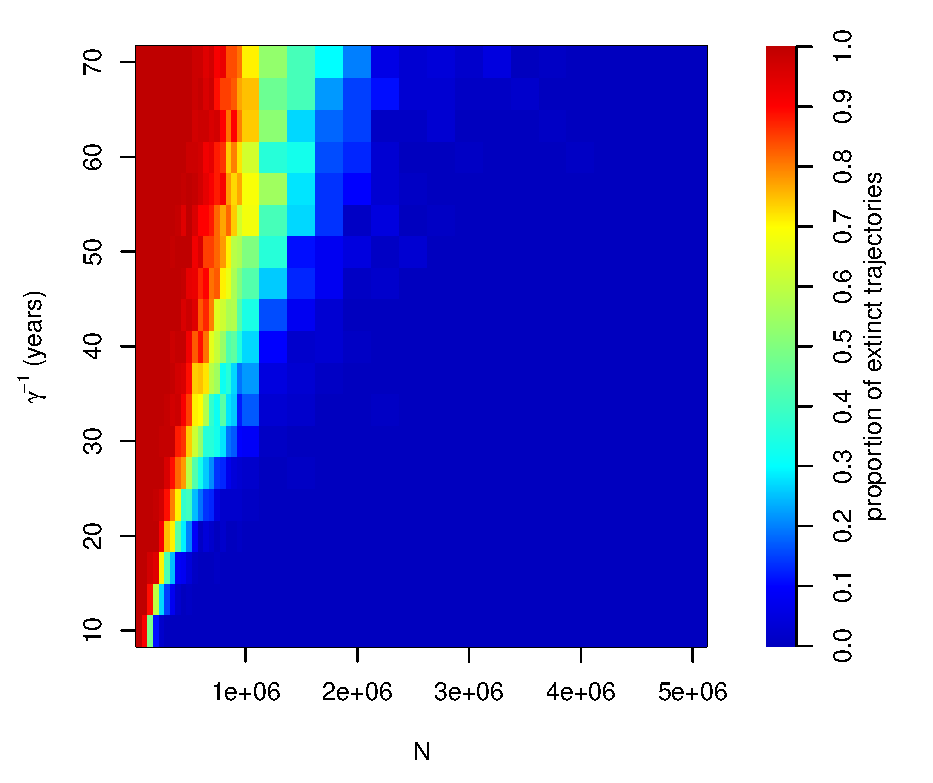
\includegraphics[width=0.5\linewidth]{graphs/article1/ccs_sirs.eps}
  \caption{Effects of gradual antigenic drift on the CCS. We do not
    explicitly model mutant strains resulting from within gradual
    antigenic drift but consider that the emergence of new viral
    strains can be captured by introducing into the model a loss of
    immunity by the host, as originally suggested by Pease (1987).
    Gradual antigenic drift is therefore modelled by a $SIRS$ model
    with demography. Parameter $\gamma$ governs the transition from
    $R$ to $S$, reproducing gradual immune escape. The proportion of
    extinct trajectories after $T_{max} = 50$ years calculated on 100
    simulations is plotted. Initial conditions correspond to the
    endemic equilibrium of the deterministic model. Parameter values
    are given in Table~1 (theoretical set).}
\label{fig:ccs_sirs}
\end{figure}

\clearpage

\section{Complementary results for the theoretical parameters set}

\begin{figure}[!h]
\center
	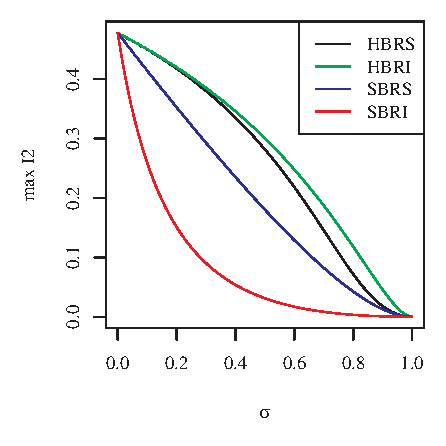
\includegraphics[]{graphs/article1/max_theoretical12.eps}
        \caption{Peak value of the first outbreak of the mutant
          cluster as a function of partial cross-immunity ($\sigma$)
          for the four models studied. Parameter values are given in
          Table 1 (theoretical set). Initial conditions are :
          ${I^1}(0) = {I^1}^*=250.4*10^{-6}$, ${I^2}(0)=10^{-6}$.}
\label{fig:max_theo}
\end{figure}


\begin{figure}[!h]
  \center
    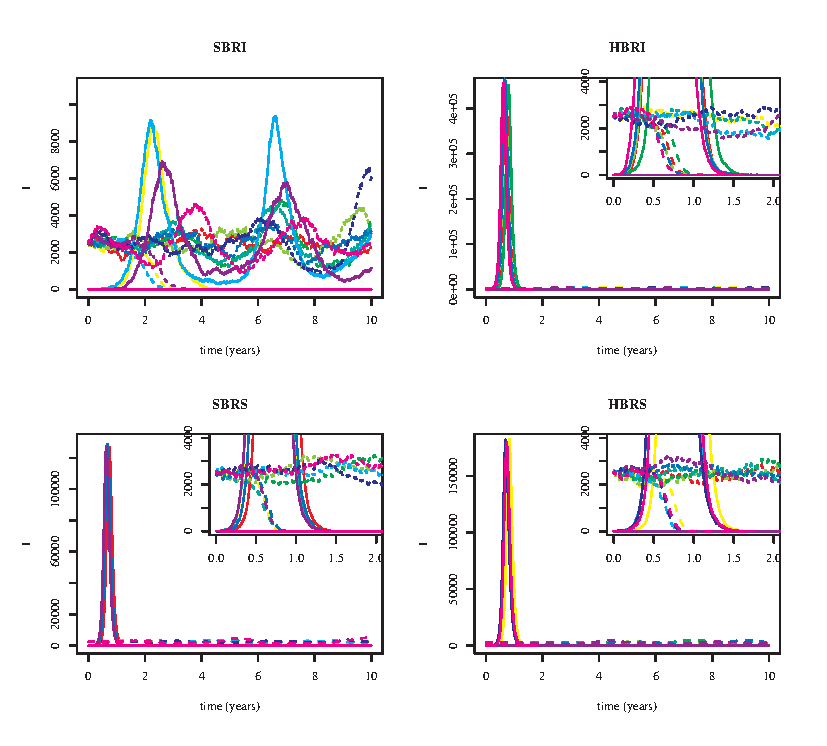
\includegraphics[width=0.8\linewidth]{graphs/article1/traj_sto_drift_theo.eps}
    \caption{Ten realisations of the four stochastic
      models for $\sigma = 0.9$ (punctuated immune escape).
      Realisations are distinguished by different colours. Plain lines
      correspond to infectious hosts for the invader antigenic cluster
      and dashed lines to infectious hosts for the resident antigenic
      cluster.}
\label{fig:sto_drift}
\end{figure}

\begin{figure}[!h]
  \center
	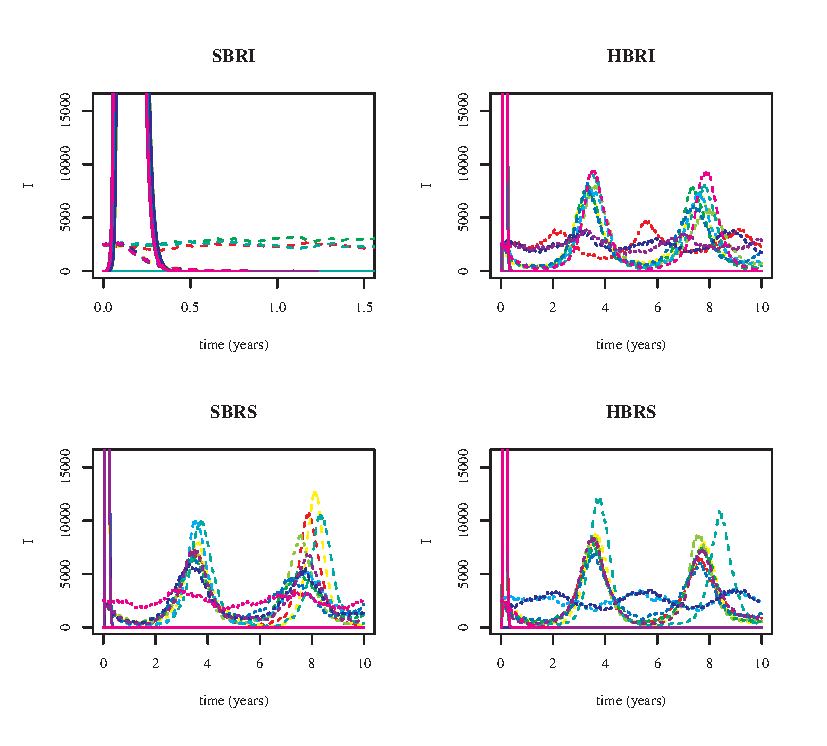
\includegraphics[width=0.8\linewidth]{graphs/article1/traj_sto_shift_theo.eps}
	\caption{Ten realisations of the four stochastic
          models for $\sigma = 0.05$ (antigenic shift). Realisations
          are distinguished by different colours. Plain lines
          correspond to infectious hosts for the invader antigenic
          cluster and dashed lines to infectious hosts for the
          resident antigenic cluster.}
	\label{fig:sto_shift}
\end{figure}


\begin{figure}[!h]
  \center
	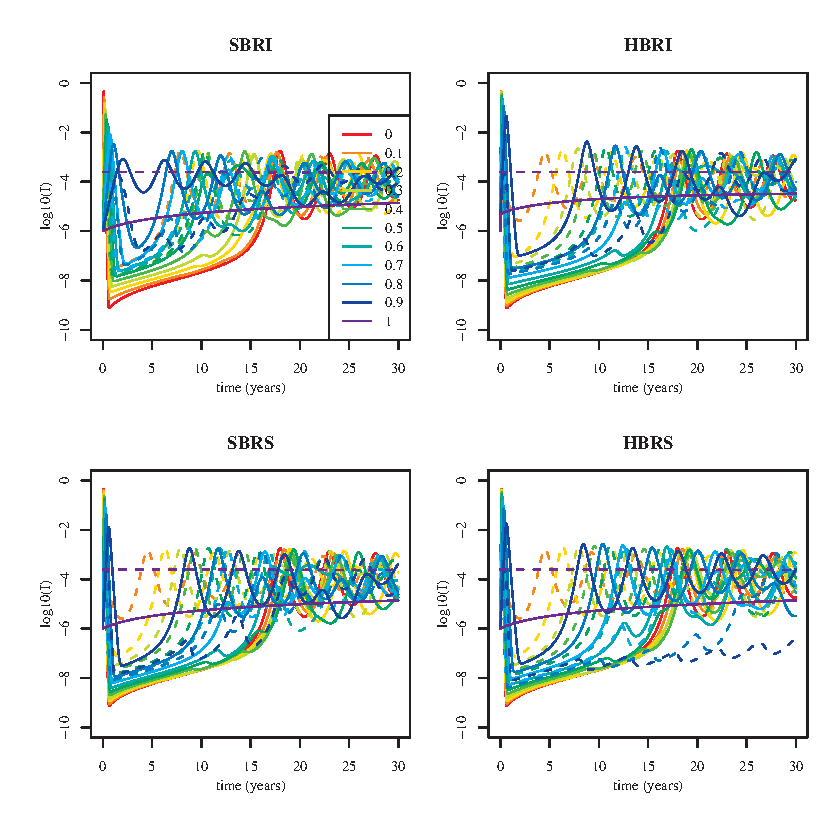
\includegraphics[]{graphs/article1/traj_sir_theoretical_migr8.eps}
	\caption{Transient invasion dynamics for the four two-cluster
          models studied in the presence of external reintroductions
          of infectious hosts. The decimal logarithm of the proportion
          of infectious hosts for the mutant antigenic cluster (plain
          lines) and for the resident cluster (dashed lines) is
          represented as a function of $\sigma$. Colours correspond to
          different partial cross-immunity ($\sigma$) values: from
          $\sigma=0$ (antigenic shift, no cross-immunity) to
          $\sigma=1$ (antigenic drift, full cross-immunity). Parameter
          values are given in Table 1 (theoretical set),
          $mp_i=10^{-8}$. Initial conditions are : ${I^1}(0) =
          {I^1}^*=250.4*10^{-6}$, ${I^2}(0)=10^{-6}$.}
	\label{fig:deter_migr}
\end{figure}

\clearpage


\section{A model for within cluster antigenic drift}

Within cluster antigenic drift is introduced by assuming that viruses
present two parts:
\begin{itemize}
\item a conserved part, identical for both clusters whose phenotype
  cannot evolve.
\item a specific part, subject to slight phenotypic variation
  following quasi-neutral mutation.
\end{itemize}

Partial cross-immunity is provided by the conserved part. Gradual
antigenic drift induces continuous changes of the specific part and,
new specific parts are introduced following immune escape mutations.
We further assume that a primary immune response results in the
acquisition of immune memory toward both the conserved and the
specific parts.

We note $\sigma$ and $\sigma_s$ ($\sigma, \sigma_s \in [0,1]$) the
degrees of protection provided respectively by immunity to the
conserved and the specific part of the virus. We assume additivity of
cross protection with the constraint that $\sigma + \sigma_s \leq 1$.

In case where we assume that within cluster antigenic drift results in
strains diversity rendering intra-cluster immunity only partial, the
previous assumption enables to recover Gökaydin \textit{et al.} (2007)
$SIRI$ model. Reinfections with strains belonging to a cluster for
which hosts have been immunised occur with a reduced probability
$(1-(\sigma+\sigma_s))$. Infections by strains belonging to a mutant
cluster never encountered by the hosts occur with a reduced
probability $(1-\sigma)$

In case where we assume that within antigenic clusters evolution
results in a progressive loss of immunity as proposed by Pease (1987)
($SIRS$ framework) we introduce a parameter ($\gamma$) governing the
rate of antigenic drift. Infections of naive hosts by strains
belonging to cluster $i$ confer full immunity toward strains of
cluster $i$ ($\sigma+\sigma_s=1$, $R_{Ci}$ hosts in figure~8 of the
main text). Antigenic drift affects the specific part of the virus
belonging to cluster $i$ and induces a loss of immunity toward the
specific part after a time governed by a rate $\gamma$ ($R_{Ci} \to
R_C$). $R_C$ hosts can then be reinfected by strains belonging to
cluster $i$ but with a reduced probability ($1-\sigma$) due to
immunity provided by the conserved part. The conserved part also
ensures that $R_{Ci}$ and $R_C$ hosts have a reduced
probability ($1-\sigma$) to be infected by strains belonging to
cluster $j$ (partial cross-immunity).

We formulate the model of figure~7 (main text) using an
$HBRS$ framework and neglecting co-infections in order to compare it
to Gökaydin \textit{et al.} (2007) model.  These assumptions lead to
the following equations:

\begin{align}
\dot{R_\varnothing} &  = \mu -\beta_1 R_\varnothing (I^1_\varnothing +
I^1_{2}) -\beta_2 R_\varnothing (I^2_\varnothing + I^2_{1}) -\mu
R_\varnothing \notag \\
\dot{I^1_\varnothing} & = \beta_1 R_\varnothing (I^1_\varnothing
+I^1_{2}) + (1-\sigma) \beta_1 R_C (I^1_\varnothing +I^1_{2}) -\nu_1
I^1_\varnothing -\mu I^1_\varnothing  \notag \\
\dot{I^1_\varnothing} & = \beta_2 R_\varnothing (I^2_\varnothing
+I^2_{1}) + (1-\sigma) \beta_2 R_C (I^2_\varnothing +I^2_{1}) -\nu_2
I^2_\varnothing -\mu I^2_\varnothing  \notag \\
%
\dot{R_{C1}} &  = \nu_1 I^1_\varnothing -(1-\sigma) \beta_2 R_{C1} (I^2_\varnothing +I^2_{1}) -\gamma_1 R_{C1} +\gamma_2 R_{C12} -\mu R_{C1}  \notag \\
\dot{R_{C2}} &  = \nu_2 I^2_\varnothing -(1-\sigma) \beta_1 R_{C2} (I^1_\varnothing +I^1_{2}) -\gamma_2 R_{C2} +\gamma_1 R_{C12} -\mu R_{C2}  \notag \\
%
\dot{R_C} &  = \gamma_1 R_{C1} + \gamma_2 R_{C2} -(1-\sigma) \beta_1
R_C (I^1_\varnothing +I^1_{2}) -(1-\sigma) \beta_2 R_C
(I^2_\varnothing +I^2_{1}) -\mu R_C   \notag \\
%
\dot{I^1_2} &  = (1-\sigma) \beta_1 R_{C2} (I^1_\varnothing +I^1_{2}) -\nu_1 I^1_2 -\mu I^1_2 \notag \\
\dot{I^2_1} &  = (1-\sigma) \beta_2 R_{C1} (I^2_\varnothing +I^2_{1}) -\nu_2 I^2_1 -\mu I^2_1 \notag \\
%
\dot{R_{C12}} &  = \nu_1 I^1_2 + \nu_2 I^2_1 -\gamma_2 R_{C12} -\gamma_1 R_{C12} -\mu R_{C12}  \notag
\end{align}


\begin{figure}[!h]
  \center
  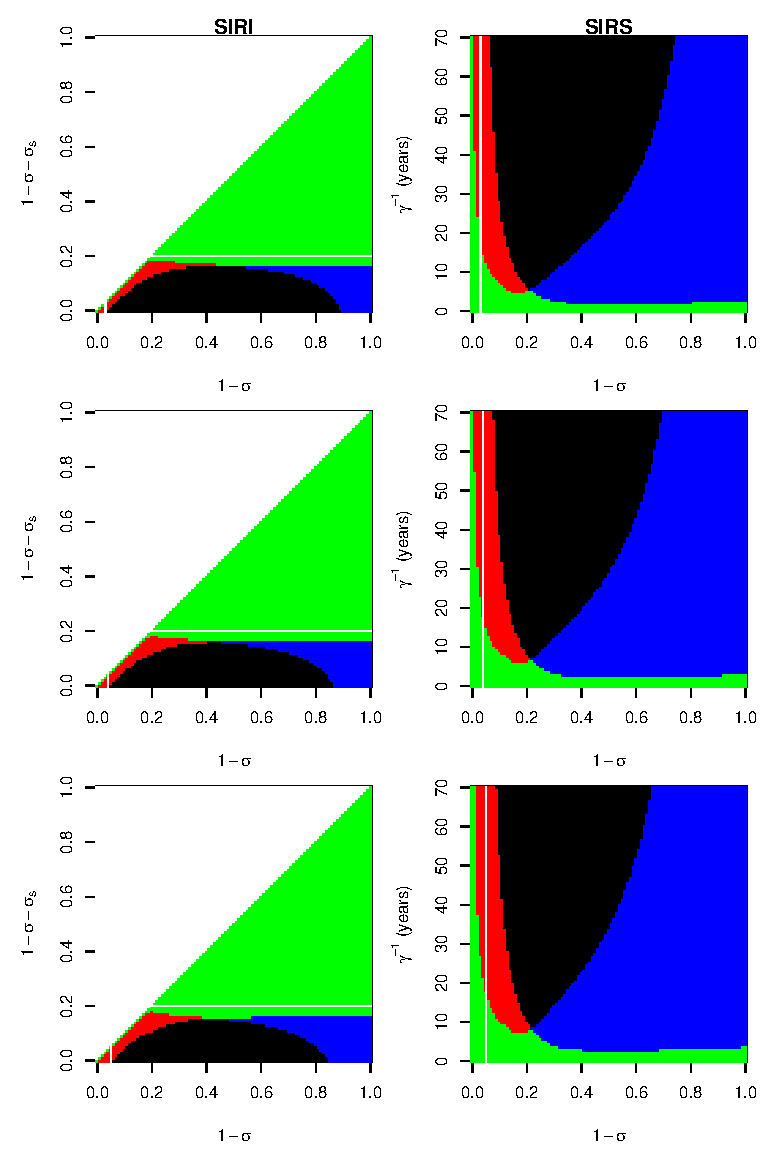
\includegraphics[width=0.5\linewidth]{graphs/article1/within_drift.eps}
  \caption{Effect of the introduction of within cluster
    gradual antigenic drift on the outcome of the invasion of a new
    antigenic cluster. Comparison of the $SIRS$ model (right)
    described in figure~7 and section 4 of the appendix with the
    $SIRI$ model of Gökaydin \textit{et al.} (2007) (left). x-axis
    scale the amount of immune escape achieved by the mutant antigenic
    cluster. y-axis represent a measure of within cluster antigenic
    drift (see section 3 of the appendix for details). Colours: both
    antigenic clusters go extinct (black), the resident cluster only
    goes extinct (successful replacement, red); the mutant cluster
    only goes extinct (blue); no cluster goes extinct (coexistence,
    green). Extinction threshold is set at $N=10^{-6}$ (top panels),
    $N=10^{-7}$ (middle panels) and $N=10^{-8}$ (bottom panels).
    Parameter values are given in Table 1 (theoretical set). The
    horizontal white lines of the right graphs situates the
    reinfections thresholds of the $SIRI$ models
    ($1-\sigma-\sigma_s=\frac{1}{R_0}$). The vertical white lines set
    the highest immune escape intensity ($1-\sigma$) for which the
    same model without within cluster antigenic drift predicts
    replacements.}
\label{fig:within_drift_app}
\end{figure}

\clearpage


\section{Functional constraints}

\begin{figure}[!h]
  \center
  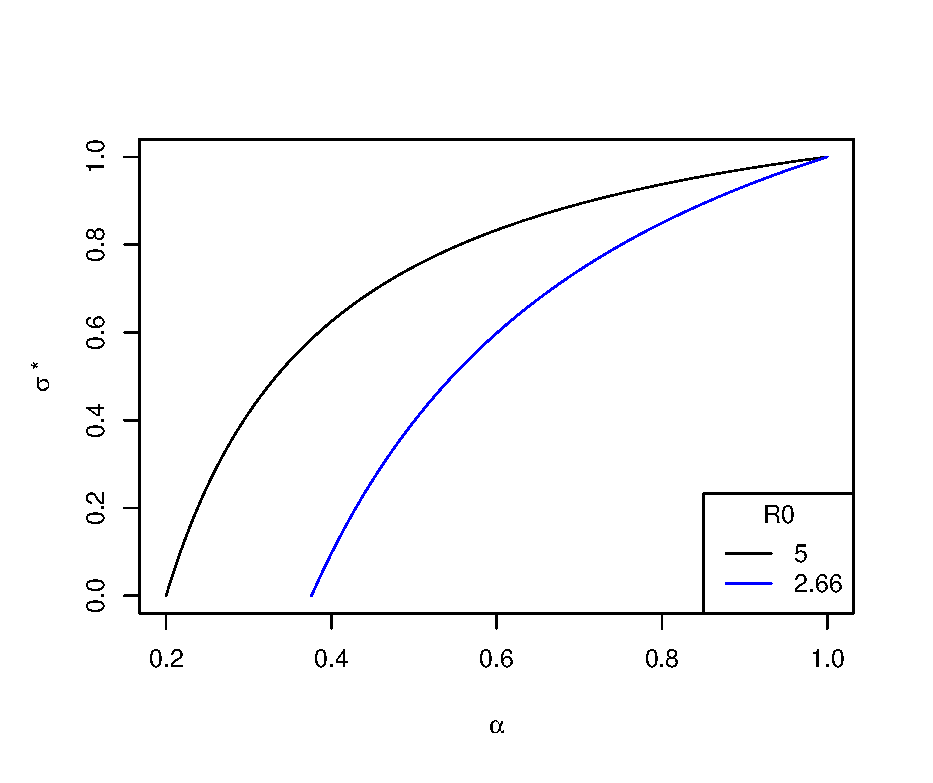
\includegraphics[width=0.5\linewidth]{graphs/article1/constraints.eps}
  \caption{Effect of the fitness reduction (mutant
    transmission rate $\beta$ reduced by a factor $\alpha$) associated
    with immune escape plotted for different values of the resident
    cluster $R_0$. The threshold value of $\sigma$ ($\sigma^*$) needed
    to ensure the mutant cluster invasion is plotted against
    $\alpha$.}
\label{fig:constraints}
\end{figure}


%\section{gupta}
%
%\begin{figure}[!h]
%  \center
%  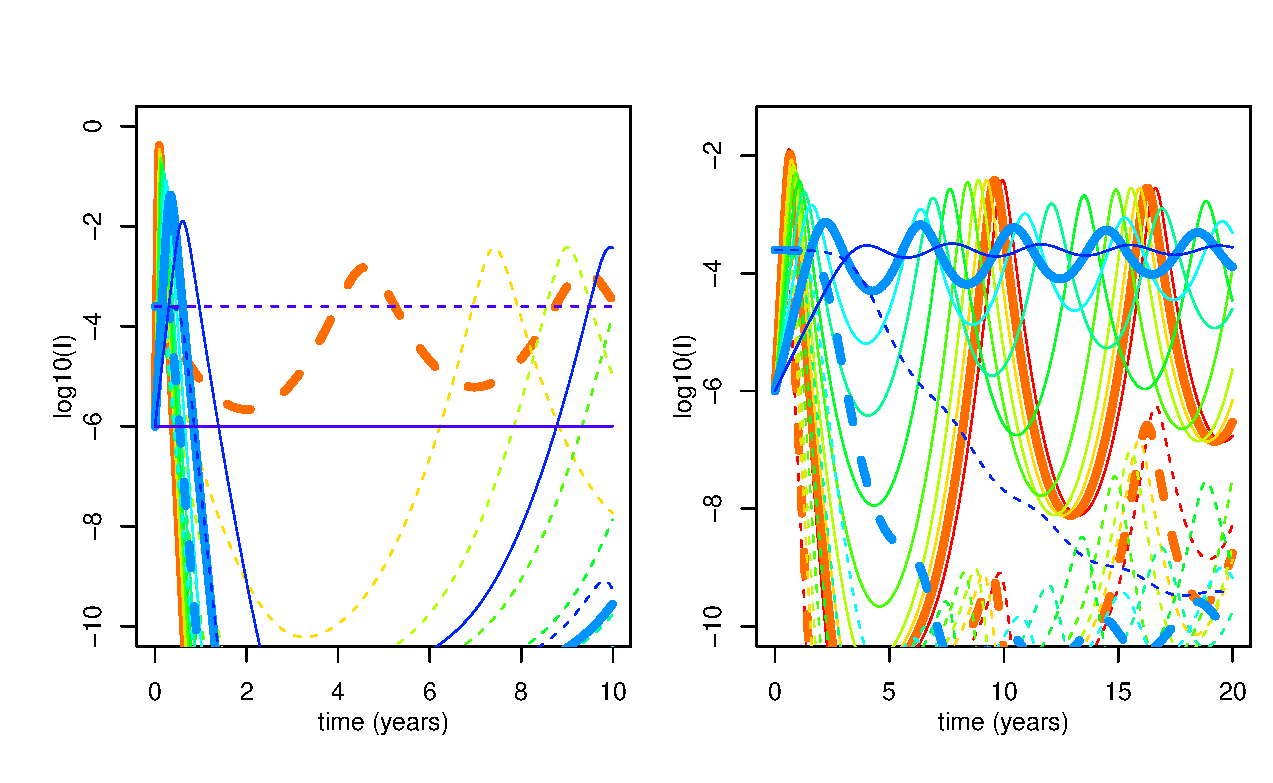
\includegraphics[width=0.9\linewidth]{gupta.eps}
%  \caption{}
%\label{fig:traj_siri2}
%\end{figure}
%
%\clearpage


%%% Local Variables: 
%%% mode: latex
%%% TeX-master: "../../phD"
%%% End: 
